\section{Simulations}

A simulation is run for the conditions stated in Theorem 1. In the simulation we have 4 agents and their initially desired $\alpha_i(0) = \pi / 3$ so the circular convergence criterion is not met, the initial positions are chosen randomly. The chosen parameters are $v=1, \mu_c=.5,\mu_s=0,\mu_r=0,\epsilon=.2$, the gain for Cyclic pursuit is chosen to be $\mu=1$ . The system converges to a circular formation with an arbitrary radius and spacing as seen in Fig \ref{fig:Adaptive}.

\begin{equation*}
  \alpha = [1.0619 \quad 0.7867 \quad 0.7939 \quad 0.4992]
\end{equation*}
\begin{figure}
	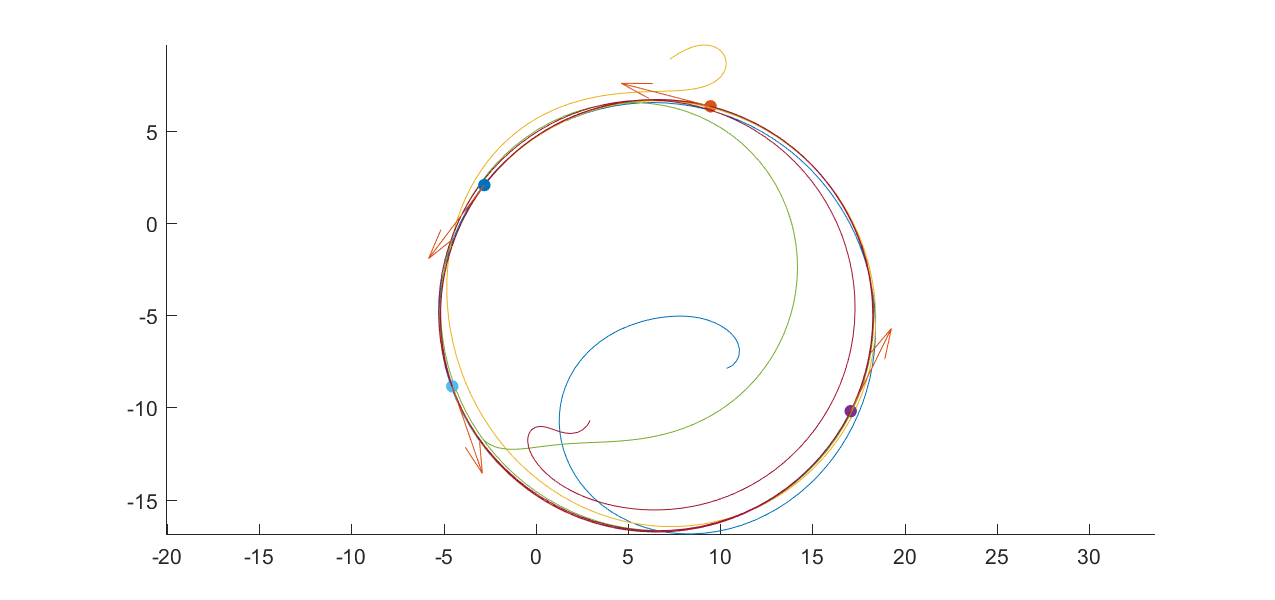
\includegraphics[width=\linewidth]{Attachments/Figure41.png}
	\caption{Circular formation with adaptive $\alpha$.}
	\label{fig:Adaptive}
\end{figure}

We now verify verify Observation 1 by simulation. The previous parameters are maintained and the radius control gain is changed to $\mu_r=.5$ and the reference radius is set to $r^*=10$. The formation now converges to a circle with a radius of 10 units as shown in Fig \ref{fig:RadiusConvergence}
\begin{figure}
	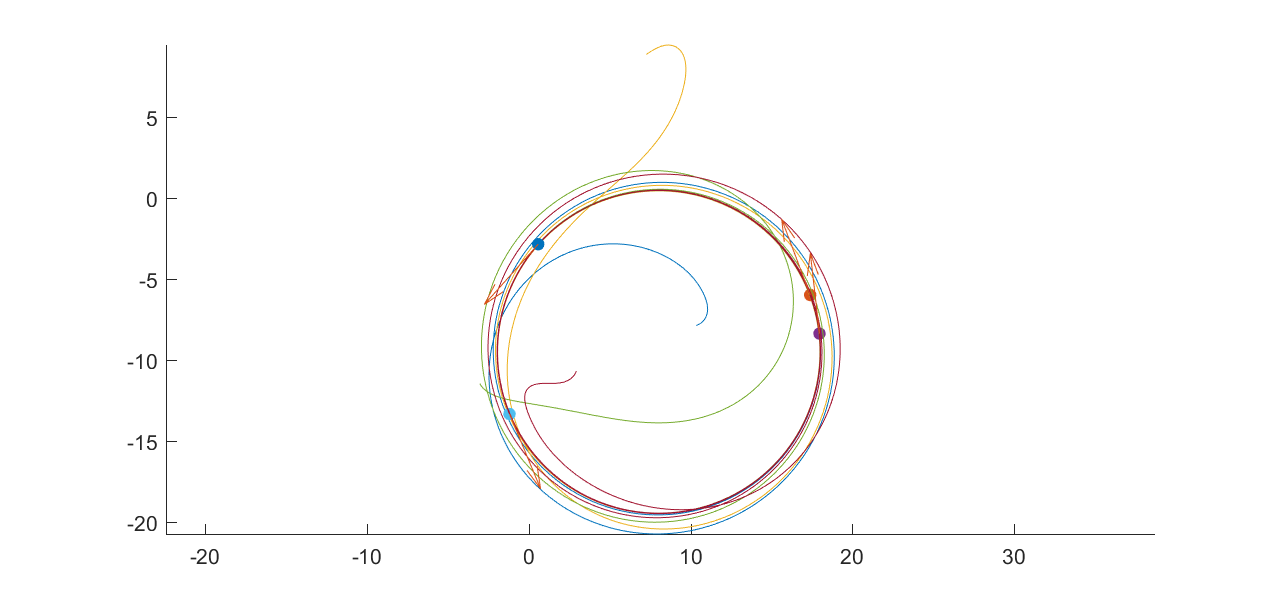
\includegraphics[width=\linewidth]{Attachments/Figure43.png}
	\caption{Circular formation with predetermined radius.}
	\label{fig:RadiusConvergence}
\end{figure}

For verifying Observation 1 the radius control gain is reverted to $\mu_r=0$. The equal spacing gain is chosen according to the guidelines provided, an order of magnitude smaller $\mu_s=.01$. The formation does not control radius but achieves an equally spaced formation as Fig  \ref{fig:EquallySpaced} shows.
\begin{figure}
	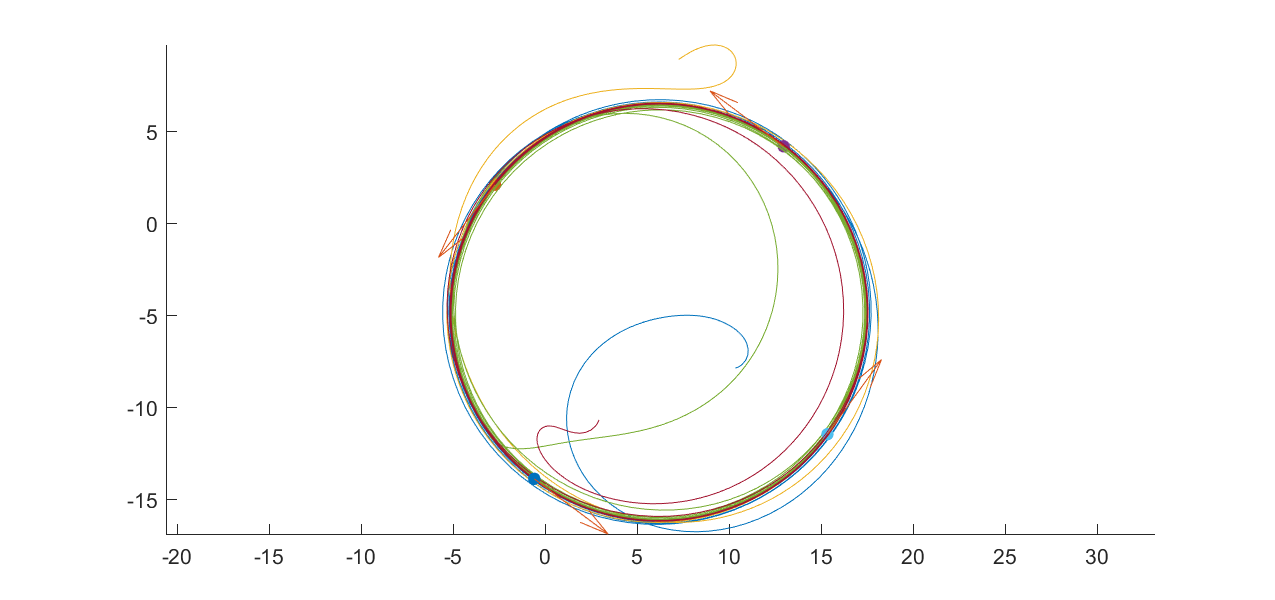
\includegraphics[width=\linewidth]{Attachments/Figure42.png}
	\caption{Equally spaced circular formation with adaptive $\alpha$.}
	\label{fig:EquallySpaced}
\end{figure}

Finally, all three control laws can be combined to achieve a circular formation with predetermined radius and equal spacing. A simulation is run with the previously used gains $\mu_c=.5,\mu_s=.01,\mu_r=.5$. The results for the complete algorithm are depicted in Fig \ref{fig:FormationConvergence}
\begin{figure}
	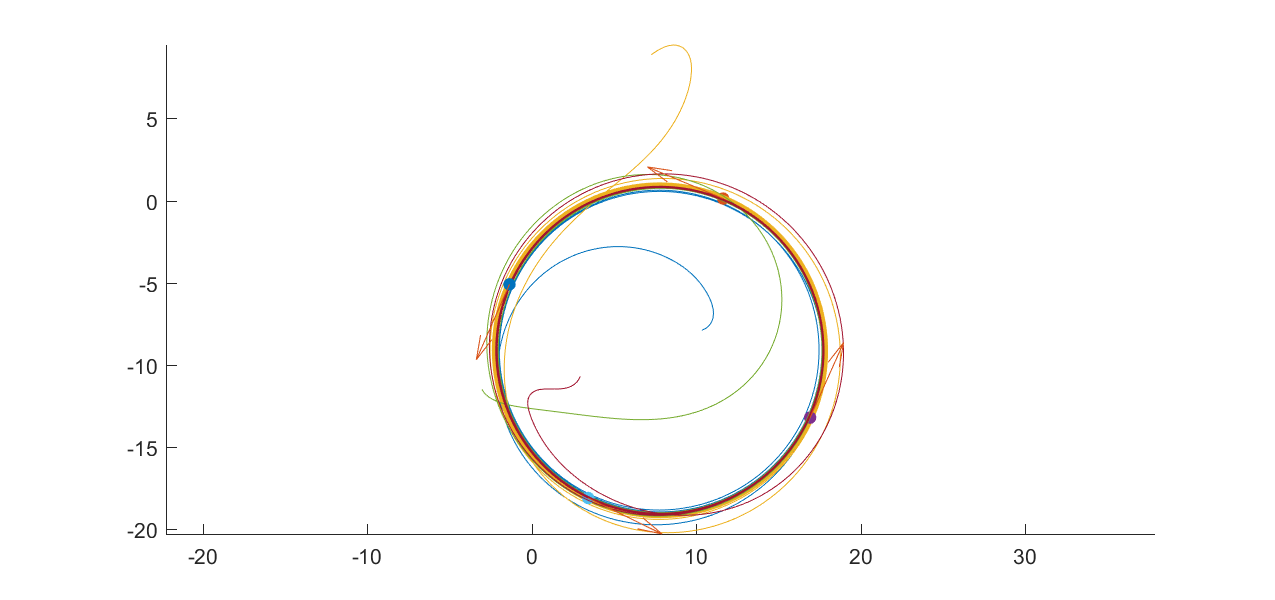
\includegraphics[width=\linewidth]{Attachments/Figure44.png}
	\caption{Equally spaced circular formation with predetermined radius.}
	\label{fig:FormationConvergence}
\end{figure}

Finally, an extra simulation is run to show the robustness of the formation to changes in the network. The following figure represents the way a formation that has already converged reacts to an agent joining the at the instant pictured in \ref{fig:Robustness}

\begin{figure}
	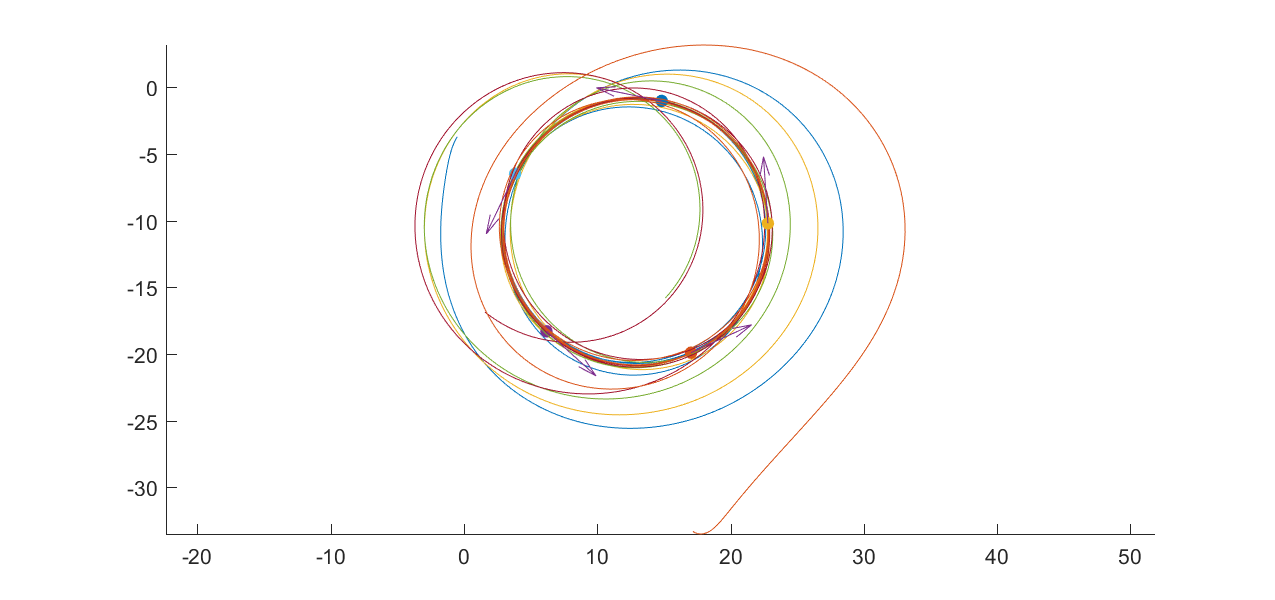
\includegraphics[width=\linewidth]{Attachments/Figure45.png}
	\caption{Robustness of the algorithm to changes in the network. The joining agent joins the formation from below.}
	\label{fig:Robustness}
\end{figure}